%% Beispiel-Präsentation mit LaTeX Beamer im KIT-Design
%% entsprechend den Gestaltungsrichtlinien vom 1. August 2020
%%
%% Siehe https://sdqweb.ipd.kit.edu/wiki/Dokumentvorlagen

%% Beispiel-Präsentation
\documentclass{sdqbeamer} 

\AtBeginSection[]{
  \begin{frame}
  \vfill
  \centering
  \begin{beamercolorbox}[]{title}
    \centering\usebeamerfont{title}\huge\underline\insertsectionhead\par%
  \end{beamercolorbox}
  \vfill
  \end{frame}
}

 
%% Titelbild
\titleimage{banner_2020_kit}

%% Gruppenlogo
%\grouplogo{mylogo} 

%% Gruppenname und Breite (Standard: 50 mm)
\groupname{Human-Computer Interaction and Accessibility}
\groupnamewidth{50mm}
\grouplogo{grouplogo.jpg}

% Beginn der Präsentation

\title[Solidarische Raumnutzung Pflichtenheft]{Kolloquium Pflichtenheft zur Solidarischen Raumnutzung}
\subtitle{PSE-Projekt WS24/25} 
\author[Soli-Gruppe]{Alexander Klee, Jannik Hönlinger, Johannes Frohnmeyer, Ben Steinle und Antonia Ammon}

\date[27.\,11.\,2024]{27. November 2024}

% Literatur 
 
\usepackage[citestyle=authoryear,bibstyle=numeric,hyperref,backend=biber]{biblatex}
\addbibresource{presentation.bib}
\bibhang1em

\begin{document}
 
%Titelseite
\KITtitleframe

%Inhaltsverzeichnis
\begin{frame}{Inhaltsverzeichnis}
\tableofcontents
\end{frame}

\section{Anforderungserhebung}

\begin{frame}{Aufgabenstellung}
    \begin{columns}
        \column{.4\textwidth}
        \begin{greenblock}{Problemstellung}
            \begin{itemize}
                \item Raum zur Verfügung
                \begin{itemize}
                    \item Ruheraum
                \end{itemize}
                \item Nur Türschild als Informationsquelle
    \end{itemize}
        \end{greenblock}
        \column{.4\textwidth}
        \begin{greenblock}{Anforderungen}
            \begin{itemize}
                \item Buchungssystem
                \item Nuancen in Bedarf dargestellt
                \item Aushandlung vereinfachen
            \end{itemize}
        \end{greenblock}
    \end{columns}
\end{frame}

\subsection{Befragungen}
\begin{frame}{\insertsubsectionhead}
    \begin{columns}
        \column{.4\textwidth}
        \begin{greenblock}{Mitarbeiter*innen}
        des HCI
        \end{greenblock}
        \begin{greenblock}{Flux}
        Hochschulgruppe für neurodivergente Menschen
        \end{greenblock}
    \end{columns}
\end{frame}

\begin{frame}{Befragung der Mitarbeiter*innen}
    \begin{itemize}
        \item Möglichkeit zur \textcolor{kit-red100}{gemeinsamen Nutzung} oder Verhandlung 
        \item Auch \textcolor{kit-cyan100}{spontane} Raumnutzung soll möglich bleiben
        \item \textcolor{kit-green100}{Übersichtlichkeit}
        \note{wenige Prios}
        \item Ruheraum
        \note{Priorität hat Funktion als Ruheraum}
        \begin{itemize}
            \item Hinweise über Verhalten
            \note{z.B. Panikattacken}
        \end{itemize}
        \item Mehrsprachig
        \item Screenreader
    \end{itemize}
\end{frame}

\begin{frame}{Befragung der Leute von Flux}
    \begin{itemize}
        \item Gut sichtbare \textcolor{kit-lightgreen100}{Statusanzeige}
        \item \textcolor{kit-orange100}{Reibungslose} Nutzung
        \item Einfaches \textcolor{kit-purple100}{Checkout}
        \begin{itemize}
            \item evtl. Hardware im Raum
        \end{itemize}
        \item Darkmode
    \end{itemize}
\end{frame}

\subsection{Anforderungen}
\begin{frame}{\insertsubsectionhead}
    \begin{itemize}
        \item Pflichten
        \item Wünsche
    \end{itemize}
\end{frame}

\begin{frame}{Pflichten}
    \begin{itemize}
        \item Web-Applikation mit KIT-Login
        \item Ansichten
        \begin{itemize}
            \item Kalender
            \item Login
            \item Termin-Erstellen
            \item Termin
            \item Terminübersicht
            \item Kontenliste
        \end{itemize}
    \end{itemize}
\end{frame}

\begin{frame}{Pflichten}
    \begin{itemize}
        \item Terminkonflikte mit Prioritäten lösen (\textcolor{kit-orange100}{reibungslos})
        \item 3 Prioritäten (\textcolor{kit-green}{Übersichtlichkeit})
        \note{info per Mail, falls termin überschrieben}
        \item Angabe, ob parallel nutzbar (\textcolor{kit-red100}{gemeinsame Nutzung})
        \note{wie genau umgesetzt bei Benutzeroberfläche}
        \item Banner mit Raumstatus (\textcolor{kit-lightgreen100}{Statusanzeige})
        \item Möglichkeit für Admin Gastkontos zu deaktivieren 
        \item Admin kann Termine löschen
    \end{itemize}
\end{frame}

\begin{frame}{Wünsche}
    \begin{itemize}
        \item Physischer Panikbutton (\textcolor{kit-purple100}{Hardware im Raum})
        \note{erstellt automatisch termin höchster priorität}
        \item Quick-Checkout/-in (\textcolor{kit-orange100}{reibungslos}, \textcolor{kit-purple100}{einfaches Checkout})
        \item Mehrere Räume möglich (Erweiterbarkeit)
        \item Hinweis auf Feiertage
        \item Termin in iCal-Format exportierbar
        \item Statistikansicht für Admins
    \end{itemize}
\end{frame}

\subsection{Was wir nicht anbieten}
\begin{frame}{\insertsubsectionhead}
    \begin{itemize}
        \item Mehrere Räume
        \note{Verteilung von Buchungen von ähnlichen Räumen usw.}
        \item Mehrere Arbeitplätze
        \item Langzeitplanung oder Buchungen länger als einen Tag
        \item Verifikation von Gastkonten
    \end{itemize}
\end{frame}

\section{Produkt}
\note{erst Benutzeroberfläche und dann 2 Beispielinterkationen für genauere Infos}

\subsection{Benutzeroberfläche}

\begin{frame}{{\insertsubsectionhead} - Kalenderansicht}
    \begin{figure}
        \centering
        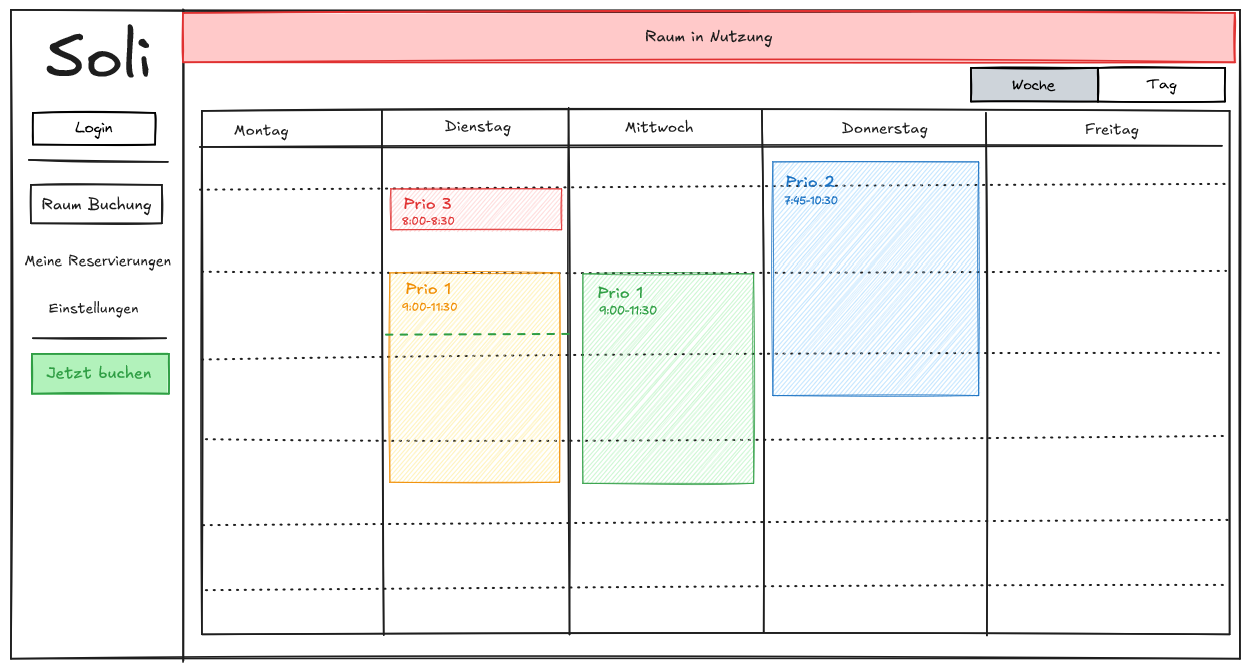
\includegraphics[width=0.75\linewidth]{Benutzeroberfläche/BenutzeroberflächeKalender.png}
        \label{fig:enter-label}
    \end{figure}
\end{frame}
\note {Übersicht über gebuchte Termine der Woche + öffnungszeiten + eigenene Termine hervorgehoben}

\begin{frame}{{\insertsubsectionhead} - Login}
    \begin{figure}
        \centering
        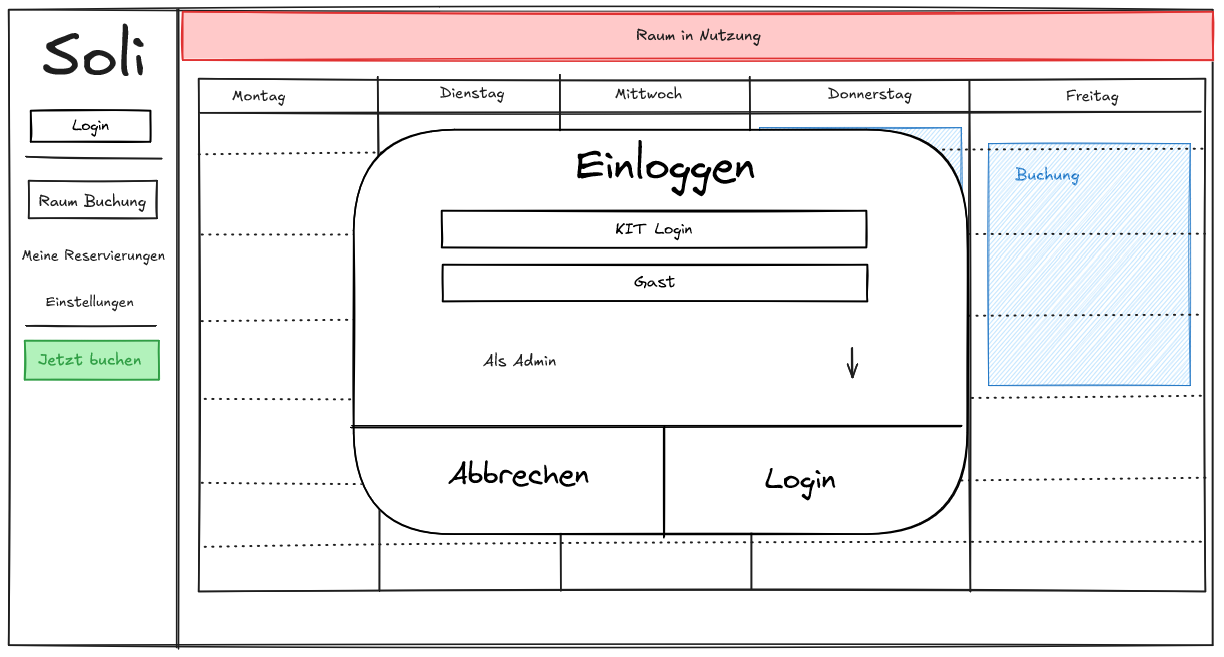
\includegraphics[width=0.75\linewidth]{Benutzeroberfläche/BenutzeroberflächeLogin.png}
        \label{fig:enter-label}
    \end{figure}
\end{frame}
\note {Login mit KIT account oder Gast auch Admin}

\begin{frame}{\insertsubsectionhead}
    \begin{figure}
        \centering
        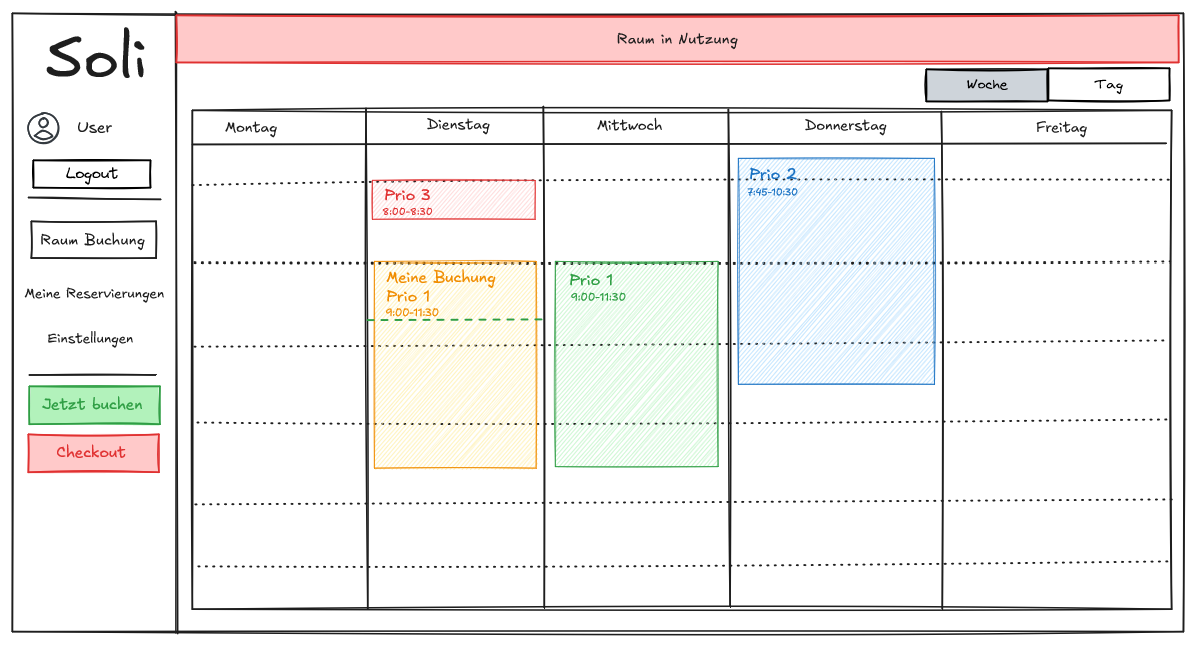
\includegraphics[width=0.75\linewidth]{Benutzeroberfläche/BenutzeroberflächeKalender2.png}
        \label{fig:enter-label}
    \end{figure}
\end{frame}
\note{wenn Buchung fertig z.B. direkt das nächste mal buchen}

\begin{frame}{{\insertsubsectionhead} - Buchen}
    \begin{figure}
        \centering
        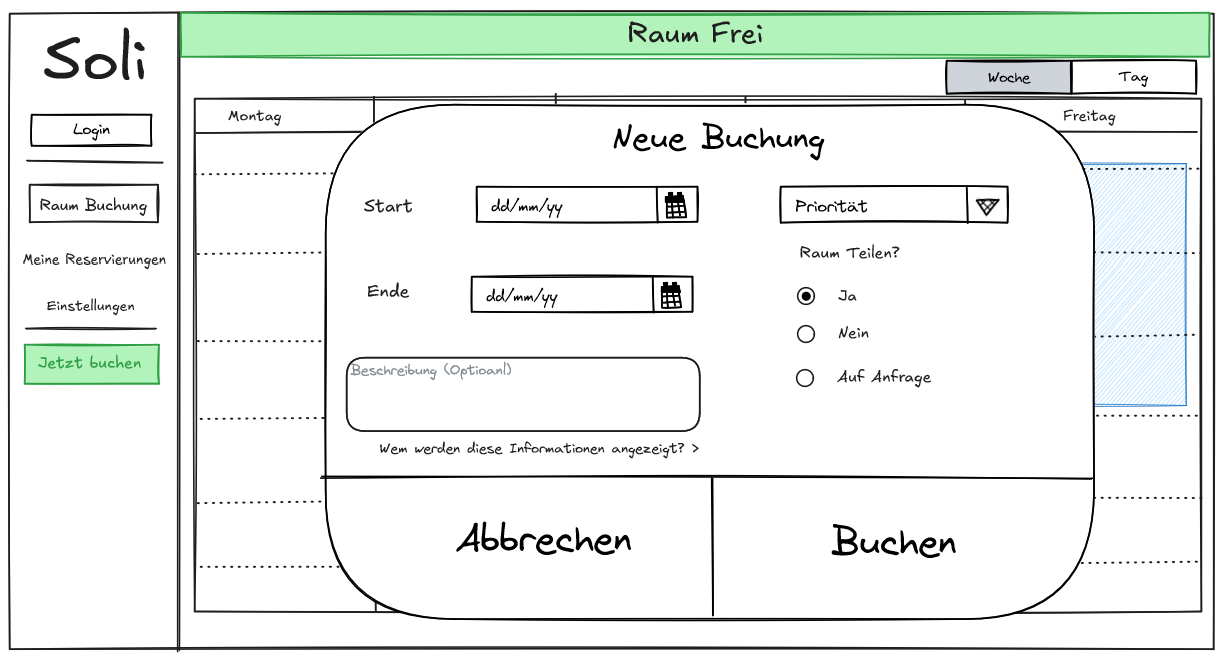
\includegraphics[width=0.75\linewidth]{Benutzeroberfläche/BenutzeroberflächeBuchung.png}
        \label{fig:enter-label}
    \end{figure}
\end{frame}
\note {neuer Termin --> aktuelle Zeit, Priorität und verhandelbarkeit + Beschreibung optional mit Hinweis}

\begin{frame}{{\insertsubsectionhead} - Terminansicht}
    \begin{figure}
        \centering
        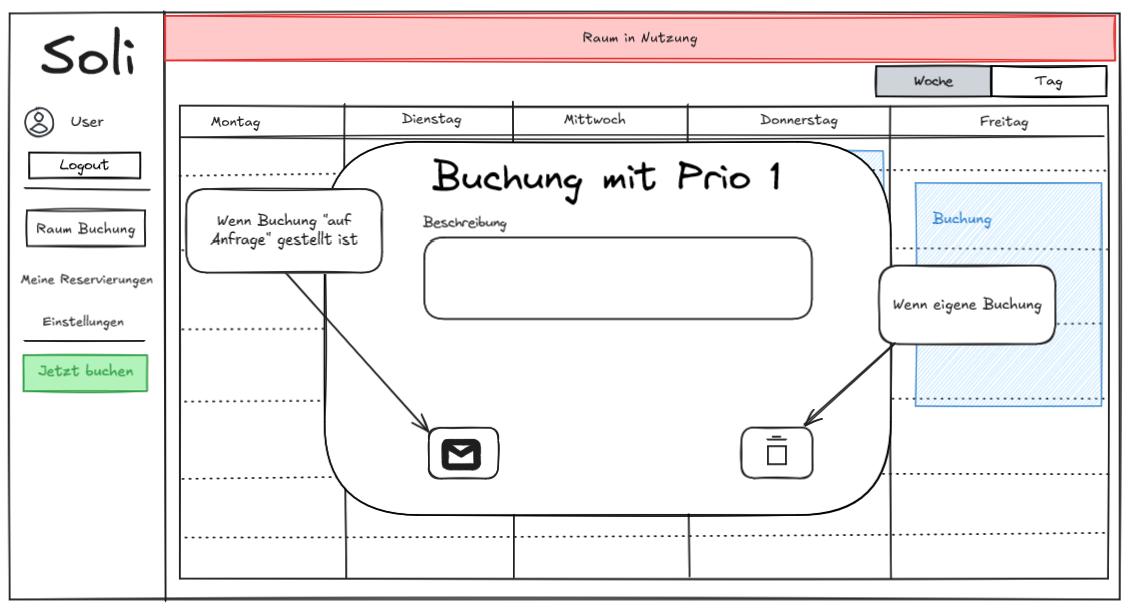
\includegraphics[width=0.75\linewidth]{Benutzeroberfläche/BenutzeroberflächeTerminansicht.png}
        \label{fig:enter-label}
    \end{figure}
\end{frame}
\note {Infos zu Termin --> wichtige Infos werden angezeit}

\begin{frame}{{\insertsubsectionhead} - Terminübersicht}
    \begin{figure}
        \centering
        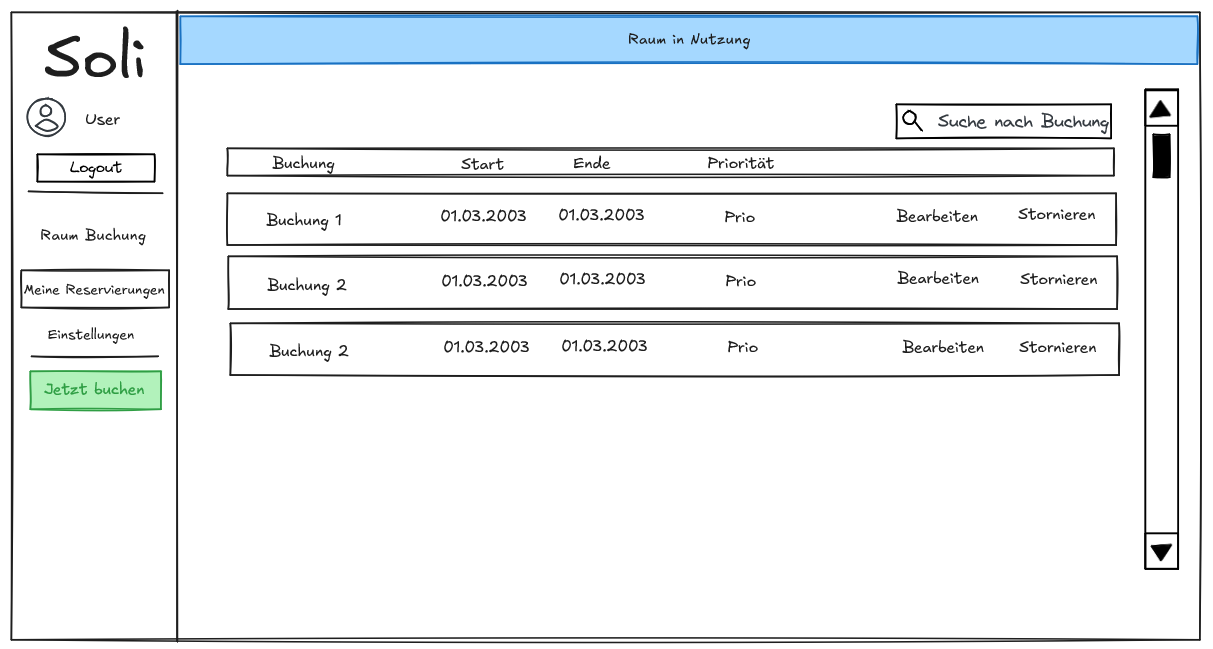
\includegraphics[width=0.75\linewidth]{Benutzeroberfläche/BenutzeroberflächeTerminübersicht.png}
        \label{fig:enter-label}
    \end{figure}
\end{frame}
\note {Auflistung der eigenen Termine zur Verwaltung}

\begin{frame}{\insertsubsectionhead - Nutzer*innenübersicht}
    \begin{figure}
        \centering
        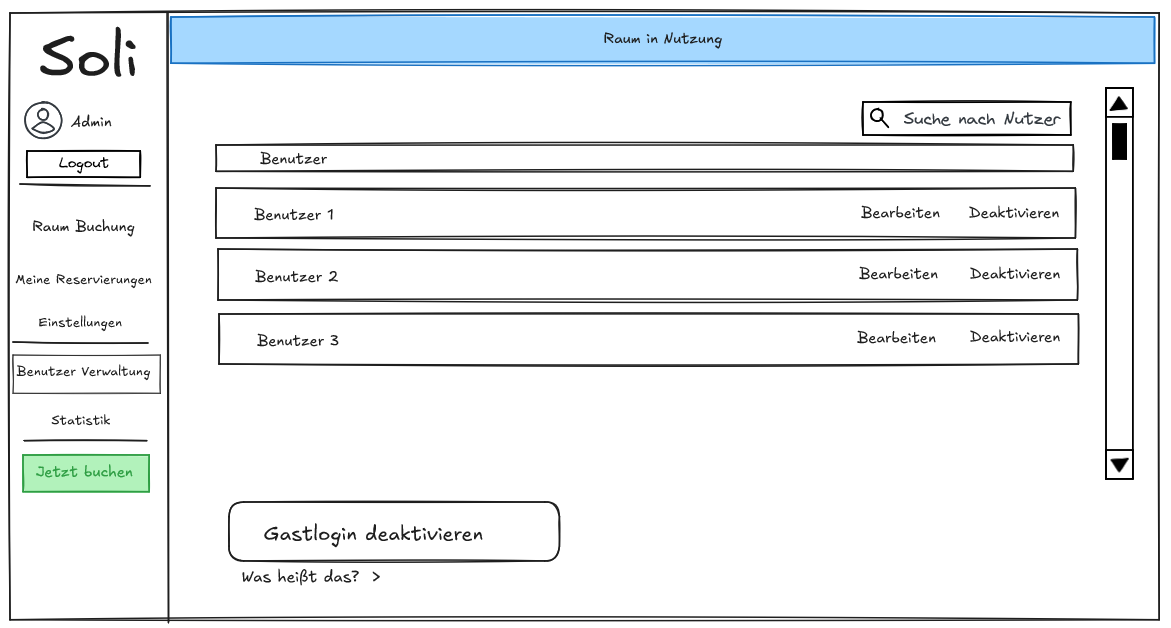
\includegraphics[width=0.75\linewidth]{Benutzeroberfläche/BenutzeroberflächeNutzerinnenansicht.png}
        \label{fig:enter-label}
    \end{figure}
\end{frame}
\note {für Admin --> Verwaltung von Konten}

\subsection{Beispielinteraktionen} 
\begin{frame}{{\insertsubsectionhead} - Anmeldefunktionalität}
    \begin{figure}
        \centering
        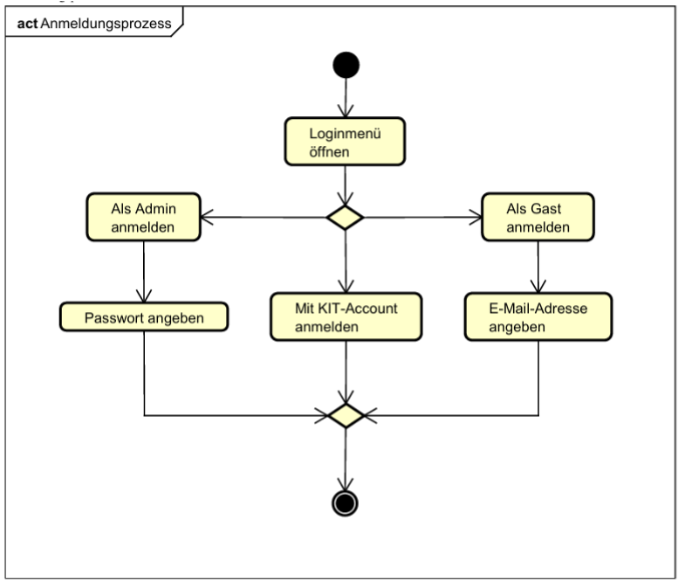
\includegraphics[width=0.5\linewidth]{Beispielinteraktionen/Anmeldung.png}
        \label{fig:enter-label}
    \end{figure}
\end{frame}

\begin{frame}{{\insertsubsectionhead} - Adminfunktionalität}
    \begin{figure}
        \centering
        \includegraphics[width=0.5\linewidth]{Beispielinteraktionen/Adminfunktionalität.png}
        \label{fig:enter-label}
    \end{figure}
\end{frame}

\subsection{Technische Umgebung}

\begin{frame}{\insertsubsectionhead}
    \begin{columns}
        \column{.4\textwidth}
        \begin{greenblock}{Entwicklungsumgebung}
            \begin{itemize}
                \item Devcontainer
                \note{reproduzierbare Entwicklungsumgebung}
                \item GitHub
                \note{z. B. Continuous Integration/Development}
            \end{itemize}
        \end{greenblock}
        \column{.4\textwidth}
        \begin{greenblock}{Hardware}
            \begin{itemize}
                \item AMD64-kompatibler Prozessor
                \item Min. 1 GB RAM
                \note{Backend}
                \item Mobiles Endgerät mit Internetzugang
                \note{frontend}
            \end{itemize}
        \end{greenblock}
    \end{columns}
\end{frame}

\begin{frame}{\insertsubsectionhead}
    \begin{columns}
        \column{.4\textwidth}
        \begin{greenblock}{Software}
            \begin{itemize}
                \item Ubuntu Linux 24.04 LTS 
                \note{Betriebssystem}
                \item Docker
                \note{Containerisierung der Anwendung}
                \item Springboot mit Java 
                \note{als Backend framework}
                \item JTE
                \note{generierung von HTML Seiten}
                \item Caddy
                \note{HTTPS-Reverse-Proxy}
                \note{und als frontend:}
                \item HTML mit Javaskript
                \item CSS-Framework
                \note{für konsistentes Design}
                \item FullCalendar
                \item Moderner Browser
            \end{itemize}
        \end{greenblock}
        \column{.4\textwidth}
        \begin{greenblock}{Schnittstelle}
            \begin{itemize}
                \item SSR
                \note{generiert statische HTML Seiten}
                \item HTML Forms
                \note{Interaktion mit Backend}
                \item Minimale REST-API
                \note{prüfen auf Verfügbarkeit}
            \end{itemize}
        \end{greenblock}
    \end{columns}
\end{frame}

\section{Q\&A}

\end{document}